\chapter{Deep Learning Side Channel Attacks}
\label{cha:dlsca}

\section{Connections to Neuro-Symbolic Learning}
\label{sec:neuro_symb}

On a high level, recall that we use PSDDs to perform tractable inference (e.g., marginalization or maximization) in the circuit product specified by
\begin{align}
    \underbrace{\pc(\mathcal{M}_B(\vv))}_{\text{Symbolic Knowledge}} \cdot \prod_{v_i \in \vv} \underbrace{\pc(p(v_i \mid \leak))}_{\text{Learned from Data}}
\end{align}
We can think of $\mathcal{M}_B$ as symbolic knowledge, while the distributions $p(v_i \mid \leak)$ are learned from data in some way (e.g., template attacks or DLSCA). This formulation is reminiscent of recent works in \emph{neuro-symbolic learning}, which focuses on bridging the fields of subsymbolic and symbolic artificial intelligence \cite{spl}. For example, Ahmed et al. have recently proposed \emph{Semantic Probabilistic Layers} (SPLs), which guarantee the output of neural networks to satisfy a constraint in a structured-output prediction problem \cite{spl}. One of their methods utilizes a PC to represent symbolic constraints via knowledge compilation techniques while using deep neural networks to output the parameters of a second PC, which are both multiplied together to constrain the support of the latter PC to assignments that satisfy the constraints \cite{spl}.

This clearly shows the similarities between our inference approach and SPL, especially when we think about $\prod_{v_i \in \vv} \pc(p(v_i | \leak))$ as a \emph{single} PC whose parameters could directly be the output of a neural network. While this circumvents the computational problem of multiplying many circuits, we find that the resulting learning problem is vastly more difficult than first learning the individual distributions $p(v_i | \leak)$. Thus, we only report experiments where we train on the latter task.

\section{Experimental Setup}
\label{sec:dlsca_exp}
% As directly parameterizing a PC as in \cite{spl} empirically does not yield satisfactory results
\begin{figure}[ht]
    % \centering
    \makebox[\textwidth][c]{
        \scalebox{0.85}{
            \begin{tikzpicture}%[trim left=5cm]
    %     \draw (0,0) rectangle node{Test} (2,2);
        \node (l) at (-2,0) {Leakage $\leak \in \mathbb{R}^{20000}$};
        \node[text width=3.5cm, align=center] (backbone) at (3,0) [draw,minimum width=1.5cm,minimum height=8cm] {Conv1D \\ ResNet \\ \vspace{0.5em} (Backbone)};
        \node (z) at (6.5,0) {$\zz$};

        \node[text width=2.5cm, align=center] (head1) at (10,3) [draw,minimum width=1.5cm,minimum height=2.2cm] {Conv1D + \\ Dense Layers \\  \vspace{0.5em} { (Head 1)}};
        \node (p_v1) at (13.5,3) {$\sigma(\zz_1) \in \mathbb{R}^d$};
        \node[text width=2.5cm, align=center] (head2) at (10,0.5) [draw,minimum width=1.5cm,minimum height=2.2cm] {Conv1D + \\ Dense Layers \\  \vspace{0.5em} { (Head 2)}};
        \node (p_v2) at (13.5,0.5) {$\sigma(\zz_2) \in \mathbb{R}^d$};
        \node (dots) at (10,-1.15) {\huge $\vdots$};
        \node[text width=2.5cm, align=center] (headn) at (10,-3.0) [draw,minimum width=1.5cm,minimum height=2.2cm] {Conv1D + \\ Dense Layers \\  \vspace{0.5em} { (Head $n$)}};
        \node (p_v3) at (13.5,-3.0) {$\sigma(\zz_n) \in \mathbb{R}^d$};

        \draw[->] (l) -- (backbone) node[midway,left] {};
        \draw[->] (backbone) -- (z) node[midway,left] {};
        \draw[->] (z) -- (head1) node[midway,left] {};
        \draw[->] (head1) -- (p_v1) node[midway,left] {};
        
        \draw[->] (z) -- (head2) node[midway,left] {};
        \draw[->] (head2) -- (p_v2) node[midway,left] {};
        
        \draw[->] (z) -- (headn) node[midway,left] {};
        \draw[->] (headn) -- (p_v3) node[midway,left] {};
\end{tikzpicture}
        }
    }%

    \caption{We use a shared backbone to produce an embedding $\zz \in \mathbb{R}^{256 \times 625}$, which is passed to $n$ heads, each producing an output $\sigma(\zz_i) \in \mathbb{R}^d$. We run two experiments: (1) We set $\sigma(\zz_i) = \softmax(\zz_i)$ and $d=256$ (\emph{byte distributions}), and (2) we set $\sigma(\zz_i) = \sigmoid(\zz_i)$ and $d=8$ (\emph{bit distributions}).}
    \label{fig:convnet}
\end{figure}

The general neural network architecture is shown in Figure \ref{fig:convnet}, is implemented in \emph{PyTorch} \cite{pytorch} and largely follows the open-source implementation\footnote{\url{https://github.com/google/scaaml}} of \cite{dlsca_defcon}. Particularly, our architecture can be classified as a \emph{Convolutional Neural Network} (CNN) \cite{cnn_fukushima, cnn_lecun}, as we make heavy use of 1D convolutional layers (\texttt{Conv1d}). Next, we describe the model architecture in more detail.

Since the \emph{Backbone} consumes a high-dimensional power trace $\leak$, we employ downsampling strategies to reduce the dimensionality of the input data: First, we utilize \emph{maximum pooling} (i.e., a \texttt{MaxPool1d} layer) with a kernel size of $4$, a stride of $4$, and a dilation of $1$. Next, we run the output of this operation to a stack of $12$ \emph{Blocks}, where each block consists of $3$ sequences of a \texttt{Conv1d} layer, followed by a \emph{Batch Normalization} layer \cite{batchnorm} (\texttt{BatchNorm1d}) and the $\relu$ activation function, defined as $\relu(x) = \max(0, x), \ x \in \mathbb{R}$ (applied elementwise). Moreover, each block uses a \emph{residual connection} as introduced in \cite{resnet}, i.e., we add the input a block receives to the output it returns. However, we slightly modify this setup and add another \texttt{Conv1d} layer to the residual connection (i.e., the input flows through a convolutional layer before being added to the output), as we find that this improves performance empirically. As common in the literature \cite{cnn_lecun}, we keep increasing the number of filters in the convolutional layers, while decreasing the dimensionality of each feature map using strides $> 0$. The final block outputs the embedding $\zz \in \mathbb{R}^{256 \times 625}$ with $256$ feature maps, each consisting of $625$ values. This embedding is then passed to the individual \emph{Heads}: Each head first runs $\zz$ through $3$ blocks (as defined above), followed by performing average pooling to produce a $512$-dimensional embedding, which is passed to a network consisting of $2$ fully connected layers (\emph{Dense} layers, often called \emph{Linear} layers) with $\relu$ activation. After the first dense layer, we again employ batch normalization using \texttt{BatchNorm1d}. The second layer outputs $\sigma(\zz_i) \in \mathbb{R}^d$ where $d=256$ and $\sigma(\zz_i) = \softmax(\zz_i)$ in our first experiment (\emph{byte distributions}) and $d=8$ and $\sigma(\zz_i) = \sigmoid(\zz_i)$ in our second experiment (\emph{bit distributions}). In both cases, we create $n=21$ heads since we wish to model the posterior distributions $p(v|\leak)$ of $21$ variables $v \in \vv$.

\begin{definition}[Softmax Activation Function]
    With $\zz = (z_1,\dots,z_d)^T \in \mathbb{R}^d$, we define
    \begin{align}
        \softmax(\zz)_i = \frac{\exp(z_i)}{\sum_{j=1}^d \exp(z_j)}
    \end{align}
    for $i \in \{1,\dots,d\}$.
    Note that $\softmax(\zz) \in \mathbb{R}^d$ is a PMF for all $\zz \in \mathbb{R}^d$.
\end{definition}

\begin{definition}[Sigmoid Activation Function]
    With $\zz = (z_1,\dots,z_d)^T \in \mathbb{R}^d$, we define
    \begin{align}
        \sigmoid(\zz)_i = \frac{1}{1 + \exp(-z_i)}
    \end{align}
    for $i \in \{1,\dots,d\}$.
    As $0 < \sigmoid(\zz)_i < 1$ for all $\zz \in \mathbb{R}^d$, we can interpret $\sigmoid(\zz)_i$ as the success parameter of a Bernoulli distribution.
\end{definition}

As a regularizer, we set each input value of the final fully connected layer to $0$ with probability $p=0.1$ during training (\emph{Dropout}). Both network architectures consist of $\approx 30$ million trainable parameters, which we fit by using the \emph{Adam} optimizer \cite{adam} with a learning rate of $0.001$ to minimize the mean of the \emph{sample losses} over $\dattrain$: Given $\leak$, the sample loss is the average cross entropy between the distributions the network outputs (i.e., $\{ \sigma(\zz_i) \}_{i=1}^n$) and the empirical distributions $p_e(v_i | \leak)$, which output $1$ if $v_i$ assumes the true value of the corresponding intermediate, and $0$ else. When $\sigma(\zz_i) = \sigmoid(\zz_i)$, we use the \emph{binary} cross entropy loss function.
For both models, we train for $30$ epochs using a batch size of $16$ and use $\datval$ to evaluate the validation loss after every epoch. We save a snapshot of the current best model (w.r.t. validation loss) to disk after every epoch and use the overall best model to perform our experiments.

\section{Experimental Results and Discussion}

\begin{figure}[h]
	\centering
	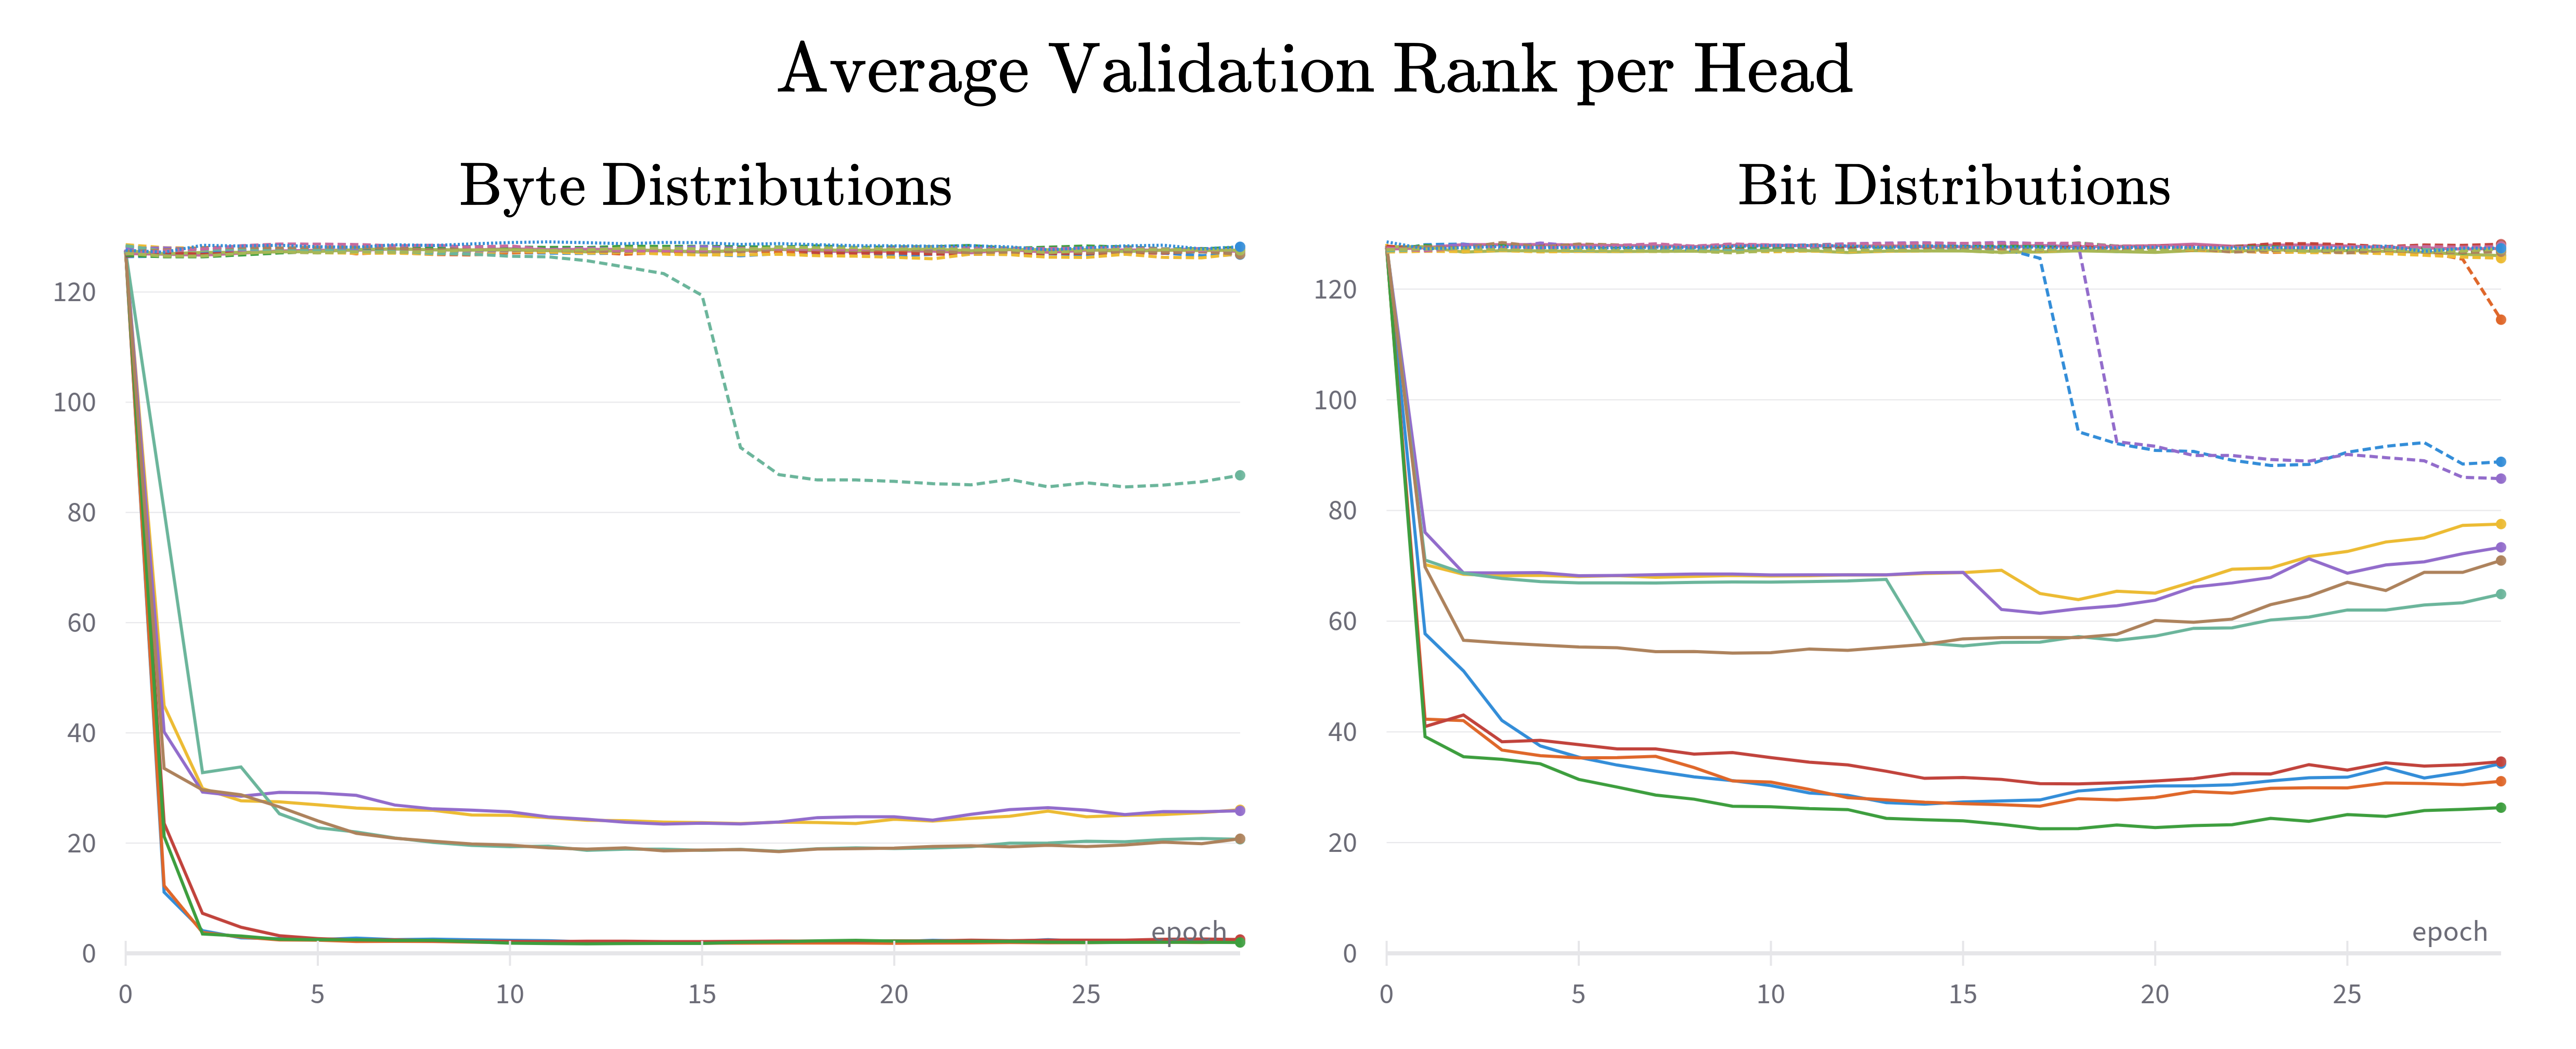
\includegraphics[width=\linewidth]{figures/average_ranks.png}
	\caption{During training, we monitor the average rank of each of the true intermediates $v \in \vv$ in the corresponding output distribution, measured on the validation set $\datval$. We observe that the fully factorized bit distributions lack the expressivity to faithfully represent the posterior distributions.}
	\label{fig:avg_rank}
\end{figure}
Figure \ref{fig:avg_rank} shows the average validation rank per head during training. We observe that some intermediates are much easier to accurately predict than others: The four heads predicting $p(v | \leak)$ for $v \in \vin$ show the lowest average validation ranks in both experiments, while many other distributions yield an average rank of $\approx 127.5$. This is the expected rank if the position of the true value is uniformly random --- effectively providing no information about the true intermediate.

More precisely, if we first use $\datval$ to calculate the mean rank of true input values $v \in \vin$ under the respective distribution the neural network predicts, i.e., $p(v | \leak)$, and average these $4$ means, we obtain an average validation rank of $2.21$ in the \emph{byte distributions} experiment, and an average validation rank of $31.58$ in the \emph{bit distributions} experiment. 

% \todo{Average ranks after inference (PSDD vs SASCA)}
We repeat the set of main experiments in Section \ref{sec:exp_isolation}, but instead of obtaining the posterior distributions $p(v | \leak)$ via template attacks, we use our neural networks to predict these distributions. In the \emph{byte distributions} experiment, we again have to sparsify the distributions $p(v | \leak) \ \forall v \in \vin$ to make the PSDD computations tractable (i.e., $\varepsilon > 0$). Note that the experimental results that follow have been obtained with $\varepsilon \in \{10^{-2}, 10^{-3}\}$, as smaller values of $\varepsilon$ made the experiments intractable.
However, as explained in Section \ref{sec:scopes}, we do not need any sparsification in the \emph{bit distribution} experiment, since PSDD multiplication is trivial when performed with circuits that represent fully-factorized Bernoulli distributions.
In order to compute a baseline and run SASCA using the predicted \emph{bit distributions} (i.e., Bernoulli parameters), we first evaluate the fully-factorized distributions for all bitstrings $x \in \mathbb{F}_2^8$ and pass the resulting PMF (with the scope of a byte, respectively) to SASCA and to the computation of the baseline (as defined in Section \ref{sec:results}).
The results of the experiments are shown in Table \ref{tab:dlsca_res}.
\begin{table}[H]
    \centering
	\begin{tabular}{|l | c | c | c | c |}
		\hline
    \multicolumn{1}{|l|}{\textbf{Inference Method}} & \multicolumn{2}{c|}{\textbf{Byte Distributions}} & \multicolumn{2}{|c|}{\textbf{Bit Distributions}} \\
    \cline{2-5}
    \multicolumn{1}{|l|}{\textbf{(MixColumns only)}} & Success Rate & Avg. Rank & Success Rate & Avg. Rank\\
		%  & \textbf{Success Rate} ($\varepsilon = 10^{-2}$) & \textbf{Average Rank} \\
	\hline %\hline
		Baseline & $43.62 \%$ & $41.54$ & $1.14 \%$ & $45.15$ \\ \hline 
		SASCA (3 BP it.)  & $42.65 \%$ & $42.30$ & $1.24 \%$ & $47.28$ \\ \hline 
		SASCA (50 BP it.)  & $61.53 \%$ & $18.13$ & $2.06 \%$ & $48.82$ \\ \hline 
		SASCA (100 BP it.)  & $61.49 \%$ & $18.48$ & $2.06 \%$ & $47.71$ \\ \hline \hline
		PSDD + MAR ($\varepsilon = 10^{-2}$) & $83.92 \%$ & $7.15$ & / & / \\ \hline 
		PSDD + MAR ($\varepsilon = 10^{-3}$) & $84.78 \%$ & $7.34$ & / & / \\ \hline 
		PSDD + MAR ($\varepsilon = 0$) & N/A & N/A & $2.70 \%$ & $44.40$ \\ \hline \hline
		PSDD + MPE ($\varepsilon = 10^{-2}$) & $92.31 \%$ & $1.60$ & / & / \\ \hline 
		PSDD + MPE ($\varepsilon = 10^{-3}$) & $\mathbf{97.03 \%}$ & $2.12$ & / & / \\ \hline 
		PSDD + MPE ($\varepsilon = 0$) & N/A & N/A & $\mathbf{10.75} \%$ & $78.40$ \\ \hline 
	\end{tabular}
	\caption{Success rate and average rank (as defined in Section \ref{sec:eval}), measured on $\dattest$. Since we only model distributions of intermediate values in \textsc{MixColumn}, these experiments can be compared to Table \ref{tab:mixcol_res} where we set $p(y_i | \leak) = \unif(\mathbb{F}_2^8) \ \forall i \in \{1,\dots,4\}$. As we do not need approximation techniques to perform exact inference using the \emph{bit distributions}, we do not run experiments with $\varepsilon > 0$ (denoted by /). Again, we denote experiments that we cannot tractably perform with N/A.}
    \label{tab:dlsca_res}
\end{table}

Interestingly, when focusing on the \emph{byte distributions} experiment, the performance gap between SASCA and the PSDD approaches is substantially larger than the gap in our main experiments: PSDD + MPE ($\varepsilon = 10^{-3}$) can successfully attack $97.03 \%$ of test traces --- amounting to $\approx 35 \%$ \emph{more} successful attacks than the best SASCA approach.

% bit dist: exact inference helps
As discussed above, the network that outputs \emph{bit distributions} is not capable of expressing the \emph{true} posterior distributions $p(v | \leak), \ v \in \vv$ well. We conclude that the assumption that these distributions factorize into individual Bernoullis is thus flawed in our attack scenario. Nevertheless, given the \emph{bit distributions}, we can perform exact inference without the need for sparsification: PSDD + MPE ($\varepsilon = 0$) can still successfully recover $10.75\%$ of the keys --- amounting to more than $5$ times as many successful attacks when compared to the best SASCA. Moreover, compared to PSDD + MAR, our results show that it is particularly beneficial to perform MPE queries against the joint in this scenario.

\chapter{Algorithms}
\section{Tractable Circuit Multiplication}
\label{app:circuit_mult}
Algorithm \ref{alg:psdd_multiplication} shows a recursive routine that takes two PSDDs $n_1, n_2$ and the vtree $v$ they both respect as input and outputs a PSDD $n$ and a constant $\kappa$ such that
\begin{align}
\forall \xx: p(\xx) = \kappa^{-1} \cdot p_1(\xx) \cdot p_2(\xx)
\end{align}
where $p_1(\xx), p_2(\xx)$ denote the distributions represented by $n_1, n_2$, respectively, and $p(\xx)$ denotes the distribution represented by the ouput PSDD $n$.
The algorithm uses a cache since a PC is not necessarily a tree, but a directed acyclic graph (DAG).

Recall that, w.l.o.g., every PSDD sum node has one or many product node children, each of which computes the product of its left child (prime) and its right child (sub). Thus, the children of every sum node $m$ can be viewed as a set of prime-sub pairs $p,s$ with corresponding weights $w$, i.e.,
\begin{align}
\text{children}(m) = \{(p_i, s_i, w_i)\}_{i=1}^k
\end{align}
where $k$ is the number of children of the $m$.
In Algorithm \ref{alg:psdd_multiplication}, we recursively traverse sum nodes of the PSDD and implicitly deal with product nodes using the notion of prime-sub-weight triplets we have just introduced.

\begin{algorithm}[ht]

    \caption{$\textsc{Multiply}$, as introduced in \cite{tractable_ops}}\label{alg:psdd_multiplication}
    \begin{algorithmic}[1]
    \Require PSDDs $n_1, n_2$, vtree node $v$ ($n_1, n_2$ are normalized w.r.t. $v$)
    \Ensure PSDD $n$, constant $\kappa$
    \If{$(n_1, n_2)$ in cache} \Comment{Check if previously computed (PC is a DAG)}
        \State $n, \kappa \gets \text{cache}(n_1, n_2)$
        \State \Return $n, \kappa$
    \EndIf
    \If{$v$ is a leaf} \Comment{$n_1$, $n_2$ are literals, Bernoullis or $\perp$}
        \If{$n_1 = \perp$ or $n_2 = \perp$ or ($n_1, n_2$ are literals and $n_1 = \neg n_2$)} 
        \State \Return $\perp, 0$ \Comment{$n_1$ and $n_2$ are incompatible}
        \ElsIf{$n_1, n_2$ are literals and $n_1 = n_2$}
        \State \Return $n_1, 1$
        \ElsIf{$n_1$ is positive literal and $n_2$ is Bernoulli}
        \State \Return $n_1, \theta(n_2)$ \Comment{$\theta(n)$ is Bernoulli parameter of $n$}
        \ElsIf{$n_1$ is negative literal and $n_2$ is Bernoulli}
        \State \Return $n_1, (1-\theta(n_2))$
        \ElsIf{$n_1$ is Bernoulli and $n_2$ is positive literal}
        \State \Return $n_2, \theta(n_1)$
        \ElsIf{$n_1$ is Bernoulli and $n_2$ is negative literal}
        \State \Return $n_2, (1-\theta(n_1))$
        \ElsIf{$n_1$ is Bernoulli and $n_2$ is Bernoulli}
        \State $\theta_1, \theta_2 \gets \theta(n_1), \theta(n_2)$
        \State \Return $n_1, \theta_1 \cdot \theta_2 \cdot (\theta_1 \cdot \theta_2 + (1-\theta_1)\cdot (1-\theta_2))^{-1}$ \Comment{Normalization}
        \EndIf
    \Else
        \State $\gamma, \kappa \gets \{\}, 0$
        \For{$(p,s, w)$ in $\text{children}(n_1)$}
            \For{$(p',s', w')$ in $\text{children}(n_2)$}
                \State $m_1, k_1 \gets \textsc{Multiply}(p, p', \text{left}(v))$ \Comment{Multiply primes recursively}
                \If{$k_1 \neq 0$} \Comment{Check if primes were compatible}
                    \State $m_2, k_2 \gets \textsc{Multiply}(s, s', \text{right}(v))$ \Comment{Multiply subs recursively}
                    \State $\eta \gets k_1 \cdot k_2 \cdot w \cdot w'$ \Comment{Compute new weights of $(m_1, m_2)$}
                    \State $\kappa \gets \kappa + \eta$ \Comment{Accumulate weights for normalization}
                    \State add $(m_1, m_2, \eta)$ to $\gamma$
                \EndIf
            \EndFor
        \EndFor
        \State $\gamma \gets \{(m_1, m_2, \eta \cdot \kappa^{-1}) \mid (m_1, m_2, \eta) \in \gamma\}$ \Comment{Normalize weights}
        \State $n \gets \text{unique PSDD node with children } \gamma$ \Comment{Cache lookup for unique nodes}
    \EndIf
    \State add $n, \kappa$ to cache
    \State \Return $(n, \kappa)$
    \end{algorithmic}
\end{algorithm}

\section{PMF to PSDD Compilation}
\label{app:pmf_to_psdd_compilation}

\begin{algorithm}[ht]
    \caption{\textsc{compile\_pmf}}\label{alg:pmf_to_psdd}
    \begin{algorithmic}[1]
    \Require Vtree $v$, PMF $p$, is\_rightmost
    \If{$v$ is a leaf}
        \If{is\_rightmost}
	    \State \Return $\left\{ \text{{node: true node, weight: 1, bitstring: null}} \right\}$
        \Else
            \State $x \gets v \text{.literal}$
	    \State \begin{varwidth}[t]{\linewidth} \Return $[ \left\{ \text{node: literal $\neg x$, weight: $p(\neg x)$, bitstring: [0]} \right\},$ \par
	    \hskip3.9em $\left\{ \text{{node: literal $x$, weight: $p(x)$, bitstring: [1]}} \right\}]$
	    \end{varwidth}
        \EndIf
    \EndIf

    \State $p_l \gets p(\text{{vars in left($v$)}})$ \Comment{Marginal distribution over left vars}
    \State $\text{nodes\_left} \gets \Call{compile\_pmf}{\text{left}(v), p_l, \text{False}}$
    \State $\text{nodes} \gets []$
    \ForAll{$n_l$ in nodes\_left where $n_l\text{.weight} > 0$}
	 \State $p_r \gets p(\text{{vars in $v$ $\mid$ vars in left($v$) = $n_l$.bitstring}})$ %\Comment{Condition on left vars}
	 \State $\text{nodes\_right} \gets \Call{compile\_pmf}{\text{right}(v), p_r, \text{is\_rightmost}}$
	 \ForAll{$n_r$ in nodes\_right where $n_r\text{.weight} > 0$}
             \State $n \gets \text{{sum node with single product child with prime $n_l$ and sub $n_r$}}$
	     \If{$n_r \text{.bitstring} \neq \text{{null}}$}
		 \State $b \gets \text{{concat $n_l\text{.bitstring}$ and $n_r\text{.bitstring}$}}$
             \Else
                 \State $b \gets \text{{null}}$
             \EndIf
	     \State add $\left\{ \text{{node: $n$, weight: $n_l\text{.weight} \cdot n_r\text{.weight}$, bitstring: $b$}} \right\}$ to nodes
         \EndFor
    \EndFor
    \If{$v$ is root or nodes\_right is singleton set with true node}
        \State $n \gets \text{{merge nodes into single sum node}}$
        \State \Return $\left\{ \text{{node: $n$, weight: 1, bitstring: null}} \right\}$
    \EndIf
    \State \Return $nodes$
    \end{algorithmic}
\end{algorithm}

Algorithm \ref{alg:pmf_to_psdd} depicts a recursive routine for compiling an arbitrary PMF $p$ to a PSDD $\pc(p)$ that respects a given vtree $v$. To start the compilation, we call $\text{res} \gets \textsc{compile\_pmf}(v, p, \text{True})$ and find the root node of $\pc(p)$ in $\text{res.node}$. Merging multiple sum nodes (with a single child) into a single sum node is achieved as follows: We collect all children and attach them to a single sum node, where the weight of each child is given by the \emph{weight} parameter in the corresponding node object.


\chapter{Proofs}
\section{Proof of Theorem \ref{theorem:tractable_marginal}}
\begin{proof}
\label{app:tractable_marginal_proof}
    Assume $p(\xx)$ to be a smooth and decomposable PC and we want to marginalize out a subset $\xx_s$. Without loss of generality, we can assume that every path from the root to a leaf is composed of \textit{alternating} sum and product nodes, starting with a sum node\footnote{If we had a PC with multiple \textit{consecutive} sum or product nodes along a path, we could easily merge them. If the root node is a product node, we can always add a unary sum node with weight 1.} with weights $w_1,\dots,w_n$. Since on the top level, $p(\xx)$ is a proper mixture of $p_1(\xx),\dots,p_n(\xx)$, we can write
    \begin{align}
        \sum_{\xx_s} p(\xx) &= \sum_{\xx_s} \sum_{i=1}^n w_i p_i(\xx) \\
                            &= \sum_{i=1}^n w_i \sum_{\xx_s} p_i(\xx)
    \end{align}
    effectively \textit{pushing} the sum $\sum_{\xx_s}$ through the sum node. Similarly, the sum $\sum_{\xx_s}$ decomposes over product nodes: Assume, w.l.o.g., that each component $p_i(\xx)$ is a product of distributions $p'_1(\xx_1),\dots,p'_k(\xx_k)$ with disjoint scopes $\xx_1,\dots,\xx_k$. Then,
    \begin{align}
        \sum_{i=1}^n w_i \sum_{\xx_s} p_i(\xx) &= \sum_{i=1}^n w_i \sum_{\xx_s} \prod_{j=1}^k p'_j(\xx_j) \\
                                               &= \sum_{i=1}^n w_i \prod_{j=1}^k \sum_{\xx_s \cap \xx_j} p'_j(\xx_j)
    \end{align}
    i.e., sums decompose into \textit{smaller} ones.
    We can repeat these two steps until we reach a leaf. Since leaves are properly normalized probability distributions, a sum over them trivially yields $1$. Consequently, to compute $\sum_{\xx_s} p(\xx)$, we replace all leaf nodes with scope $\in \xx_s$ with a constant $1$ and perform a \textit{single forward pass} (i.e., we follow the computational graph from leaves to root), collecting the exact marginal at the root node.
\end{proof}

\section{Proof of Theorem \ref{theorem:tractable_mpe}}
\label{app:tractable_mpe_proof}
\begin{proof}
    Assume a PC $p(\xx)$ to be smooth, decomposable, and deterministic. Due to determinism, every sum node has at most one child that evaluates to a non-zero value and contributes to the sum. Consider a sum node with children $p_1(\xx),\dots,p_n(\xx)$ and weights $w_1,\dots,w_n$. Then, we can write
    \begin{equation}
        \sum_{i} w_i p_i(\xx) = \max_{i} w_i p_i(\xx)
    \end{equation}
    If we want to maximize the mixture, we can use this fact to \textit{push} the $\max$ operation through the sum node:
    \begin{align}
        \max_{\xx} \sum_{i} w_i p_i(\xx) &= \max_{\xx} \max_{i} w_i p_i(\xx) \\
                                         &= \max_{i} \max_{\xx} w_i p_i(\xx)
    \end{align}
    When encountering a product node with children $p'_1(\xx_1),\dots,p'_k(\xx_k)$ with disjoint scopes $\xx_1,\dots,\xx_k$, we see that
    \begin{align}
        \max_{\xx} \prod_{j} p'_j(\xx_j) &= \prod_{j} \max_{\xx_j} p'_j(\xx_j)
    \end{align}
    As a consequence, we can recursively push the $\max$ operation from the root node to the leaves. When the leaf is a simple parametric distribution, computing its maximum (or the maximizing argument) is usually trivial (e.g., Bernoulli, Gaussian).
    To summarize, to compute $\max_{\xx} p(\xx)$, we replace all leaf nodes with the maximum value it can assume and compute a \textit{single forward pass} while replacing all sum nodes with $\max$ nodes. To find $\argmax_{\xx} p(\xx)$, we can use the same algorithm, but also track the arguments that maximize a node.
\end{proof}

\section{Proof of Theorem \ref{theorem:kl}}
\label{app:kl_proof}
\begin{proof}
Let $p(\vv) = \prod_{j=1}^K p^{(j)}(v_j)$ and let $\mathcal{V}_j$ be the set of values $v$ such that the $\pi$-sparse approximation $\tilde{p}_\pi^{(j)}(v)$ assigns positive mass to $v$ (i.e., its support)\footnote{We omit conditioning on $\leak$ for succinctness.}. More precisely, the relation between the $j^{\text{th}}$ input distribution $p^{(j)}$ and its approximation is given by
\begin{align}
\tilde{p}_\pi^{(j)}(v) = 
\begin{cases}
    p^{(j)}(v) \cdot Z_j^{-1} \quad \text{if } v \in \mathcal{V}_j \\
    0 \quad \text{else}
\end{cases}
\end{align}
with $Z_j = \sum_{v \in \mathcal{V}_j} p^{(j)}(v)$.
As defined in Theorem \ref{theorem:kl}, let $\mathcal{J} \subseteq \{1,\dots,K\}$ denote the set of $k$ indices of $\pi$-sparse approximations and recall that
\begin{align}
    \tilde{p}(\vv) = \prod_{j \in \mathcal{J}} \tilde{p}^{(j)}_\pi(v_j) \cdot \prod_{j \notin \mathcal{J}} p^{(j)}(v_j)
\end{align}
Note that for arbitrary PMFs $q(\xx), q'(\xx), r(\yy)$ over disjoint sets of variables $\xx, \yy$, we have
\begin{align}
    D_{KL}\left( q(\xx) r(\yy) \ || \ q'(\xx) r(\yy) \right) &= \sum_{\xx} \sum_{\yy} q(\xx) r(\yy) \cdot \log \left( \frac{q(\xx) r(\yy)}{q'(\xx) r(\yy)} \right) \\
    &= \sum_{\xx} q(\xx) \log \left( \frac{q(\xx)}{q'(\xx)} \right) \cdot \sum_{\yy} r(\yy) \\
    &= D_{KL}\left( q(\xx) \ || \ q'(\xx) \right)
\end{align}
i.e., identical factors cancel in the computation of the KL-divergence. Thus,
\begin{align}
    D_{KL}\left( \tilde{p}(\vv) \ || \ p(\vv) \right) &= D_{KL}\left( \prod_{j \in \mathcal{J}} \tilde{p}^{(j)}_\pi(v_j) \ || \ \prod_{j \in \mathcal{J}} p^{(j)}(v_j) \right)
\end{align}

Let $Z = \prod_{j \in \mathcal{J}} Z_j$ and $\mathcal{V} = \mathcal{V}_{j_1} \times \dots \times \mathcal{V}_{j_k}$ where $\mathcal{J} = \{ j_1,\dots,j_k \}$. We will make use of the fact that $\forall \vv = (v_{j_1}, \dots, v_{j_k})^T \in \mathcal{V}$, we have
\begin{align}
\prod_{j \in \mathcal{J}} \tilde{p}^{(j)}_\pi(v_j) &= \prod_{j \in \mathcal{J}} \frac{1}{Z_j} p^{(j)}(v_j) \\
&= \frac{1}{Z} \prod_{j \in \mathcal{J}} p^{(j)}(v_j)
\end{align}
Expanding the KL-divergence via its definition, we can heavily simplify:
\begin{align}
    D_{KL}\left( \tilde{p}(\vv) \ || \ p(\vv) \right) &= D_{KL}\left( \prod_{j \in \mathcal{J}} \tilde{p}^{(j)}_\pi(v_j) \ || \ \prod_{j \in \mathcal{J}} p^{(j)}(v_j) \right) \\
    &= \sum_{\vv \in \mathcal{V}} \prod_{j \in \mathcal{J}} \tilde{p}^{(j)}_\pi(v_j) \cdot \log \left( \frac{\prod_{j \in \mathcal{J}} \tilde{p}^{(j)}_\pi(v_j)}{\prod_{j \in \mathcal{J}} p^{(j)}(v_j)} \right) \\
    &= \sum_{\vv \in \mathcal{V}} \frac{1}{Z} \prod_{j \in \mathcal{J}} p^{(j)}(v_j) \cdot \log \left( \frac{\frac{1}{Z} \prod_{j \in \mathcal{J}} p^{(j)}(v_j)}{\prod_{j \in \mathcal{J}} p^{(j)}(v_j)} \right) \\
    &= \sum_{\vv \in \mathcal{V}} \frac{1}{Z} \prod_{j \in \mathcal{J}} p^{(j)}(v_j) \cdot \log \left( \frac{1}{Z} \right) \\
    &= \frac{-\log(Z)}{Z} \prod_{j \in \mathcal{J}} \sum_{v_j \in \mathcal{V}_j} p^{(j)}(v_j) \\
    &= \frac{-\log(Z)}{Z} \prod_{j \in \mathcal{J}} Z_j = \frac{-\log(Z)}{Z} Z = -\log(Z)
\end{align}
By construction of the approximations, we have $Z_j \geq \pi, \forall j \in \mathcal{J}$:
\begin{align}
-\log(Z) &= -\log \left( \prod_{j \in \mathcal{J}} Z_j \right) \\
         &\leq -\log \left( \pi^k \right) = -\log \left( \pi \right) \cdot k
\end{align}
\end{proof}

\section{Proof of Theorem \ref{thoerem:ff_pc}}
\label{app:ff_pc}
\begin{proof}
Let $v$ be a vtree over variables $x_1,\dots,x_n$. To construct a PC representation of $p(\xx) = \prod_{i=1}^n p(x_i)$ that respects $v$, we will transform $v$ into a PC as follows: Replace every internal node in $v$ with a product node and every leaf in $v$ (denoted $x_i$) with a Bernoulli distribution with success parameter $\theta_i = p(x_i)$. Since the resulting PC has no sum nodes, the circuit is trivially smooth and deterministic\footnote{Clearly, these properties hold even if we introduce unary sum nodes.}. Since $v$ is a tree and the leaves of $v$ are in a one-to-one correspondence to the variables $x_1,\dots,x_n$, every internal node in $v$ must have variables in its left subtree $\xx_l$ and variables in its right subtree $\xx_r$ such that $\xx_l \cap \xx_r = \emptyset$. Therefore, the resulting circuit is decomposable. Further, the PC is, trivially, structured decomposable since each product node has a unique scope. As $v$ is a full binary tree, it has $2n - 1 \in O(n)$ nodes and $2n - 2 \in O(n)$ edges. As every node and edge is visited exactly once in the construction process of the PC, the time and space complexity of this algorithm is $\in O(n)$ (assuming that creating nodes and edges in a PC is a constant time operation).
\end{proof}

\section{Proof of Theorem \ref{thoerem:ff_pc_mult}}
\label{app:ff_pc_mult}
\begin{proof}
As $p_2$ has a single node for every vtree node, the inner loop in Algorithm \ref{alg:psdd_multiplication} (that loops over $\text{children}(n_2)$) collapses to a single iteration. As it can be shown that Algorithm \ref{alg:psdd_multiplication} visits every node in $p_1$ exactly once \cite{tractable_ops}, the resulting time complexity is $O(s_1)$. If $s_2$ denotes the size of $p_2$, we also note that $s_1 \geq s_2$ as $p_2$ is the smallest PSDD that respects the corresponding vtree.
\end{proof}